\documentclass[12pt]{paper}
\usepackage[english]{babel}
\usepackage{indentfirst}
\usepackage{graphicx}
\usepackage{latexsym}
\usepackage{amsmath}
\usepackage{amsthm}
\usepackage{amssymb,amsfonts}
\usepackage{multicol}
\usepackage{xcolor}
\usepackage{changepage}
% \usepackage{hyperref}
\usepackage{fancyhdr}
% \usepackage{showkeys}
\usepackage{textcomp}
\usepackage{mathtools}
\usepackage{comment}
\usepackage[normalem]{ulem}
\usepackage{marginnote}
%%%%%
\mathtoolsset{showonlyrefs=false}

\newcommand{\ga}{\alpha}
\newcommand{\gb}{\beta}
\newcommand{\gam}{\gamma}
\newcommand{\gd}{\delta}
\newcommand{\eps}{\epsilon}
\newcommand{\veps}{\varepsilon}
\newcommand{\gz}{\zeta}
\newcommand{\gt}{\theta}
\newcommand{\gi}{\iota}
\newcommand{\gk}{\kappa}
\newcommand{\gl}{\lambda}
\newcommand{\gs}{\sigma}
\newcommand{\go}{\omega}
\newcommand{\Gam}{\Gamma}
\newcommand{\gD}{\Delta}
\newcommand{\gT}{\Theta}
\newcommand{\gL}{\Lambda}
\newcommand{\gS}{\Sigma}
\newcommand{\gO}{\Omega}

%%%%%%%%%

\newcommand{\pt}[1]{\left( #1\right)}
\newcommand{\pq}[1]{\left[ #1 \right]}
\newcommand{\pg}[1]{\left\{ #1\right\}}
\newcommand{\figref}[1]{\figurename~\ref{#1}}
\newcommand{\red}[1]{\textcolor{red}{#1}}
\newcommand{\blue}[1]{\textcolor{blue}{#1}}
\newcommand{\gray}[1]{\textcolor{gray}{#1}}
%%%%%%%%%


\setlength{\textheight}{20cm}
%\changetext{0cm}{0cm}{0cm}{0cm}{0cm}
\changepage{2.5cm}{3.0cm}{-4cm}{-1.0cm}{-2cm}{-2cm}{-0.6cm}{0.5cm}{0cm}
%{length of the text}{width of the text}{}{shift to the right}
%{}{}{}{}{from text to pagenumber}
%\pagenumbering{roman}
\pagestyle{fancy}
\lhead{\bf \today}
\chead{\bf HP world}
\rhead{ \begin{bf}EG,KD\end{bf}}
\title{HP world paper: March 19, 2015 -- \today}
\author{}
\date{\today}

\begin{document}
 \maketitle
 \tableofcontents
 \includecomment{comment}
 
 \section*{COLOR CODE}
\paragraph{\textcolor{blue}{Blue: } reformulate}
\paragraph{\red{Red: }comments, todo}

 
\section{Introduction} 

% \marginnote{\red{Background Statement}} 
\textbf{Functioning of modern organisms is not possible nucleic 
acids and proteins.} Cells produce these extremely long polymers with cell machinery 
like ribosomes and polymerases -- also extremely long polymers. 
Therefore question ``how long 
polymers can be produced prebiotically?'' is crucial for the origin of life research.
we know that amino acids can be produced prebiotically \cite{Miller1953} and are abundant in 
stony meteorites \cite{Sephton2002}; significant progress has been made in synthesis of 
single nucleotides \cite{Powner2009a}. \textbf{However a discovery of a mechanism of prebiotic 
production of biochemically 
long polypeptides or nucleic acids despite certain success 
\cite{Shock1992,Martin1998,PAECHT-HOROWITZ1970,Lambert2008,Leman2004a,Orgel2004,Ferris1996} is 
still in the future.}

Spontaneous polymerization processes fall under what we call Flory problem (for details see 
sec.\ref{sec:flory}): chain length follow exponential distribution and desirably long chains are 
present in negligible quantities. While increasing equilibrium constant by means of catalysis or 
changing conditions to dry medium would lead to longer chain lengths, it will still give 
exponentially decreasing distribution of length. We show the proof of it for the case of monomer 
addition in \ref{sec:flory-derivation}. The proof for polymer concatenation is present in 
\cite{Derr2012}. This dynamics can be observed even in some autocatalytic systems \cite{Wu2009}.

This suggests that first catalysts emerged from mixture of short sequences, which were both 
not diverse and had poor information content. Therefore the problem of short chains also brings 
with itself problems of information production and complexity emergence \cite{Joyce1987,Abel2005}

 We sought a simple structure based mechanism, 
which would solve Flory problem, which would be able to select for certain sequences and 
amplify their chain lengths.

 We present here a physical mechanism, which give rise to 
heavy tail chain lengths distribution and selects the sequences based on the physical principle: 
hydrophobic interaction. 
\red{write about autocatalytic sets here and cite Kauffman, maybe also mention far from 
equilibrium statement.}
Our \textit{in-silico} experiments demonstrate that binary polymers 
capable of primitive folding and hydrophobic interaction is a working mechanism. Not only we get 
longer chains and selection. Our systems gives reasonable computational diversity of the sequences.


   
\section{Flory problem}\label{sec:flory}
In the systems with spontaneous polymerization chain lengths of the produced polymers follow 
exponential (Flory) distribution (see fig. \ref{fig:flory} and appendix section 
\ref{sec:flory-derivation}).

\begin{figure}[h!]
  \centering
  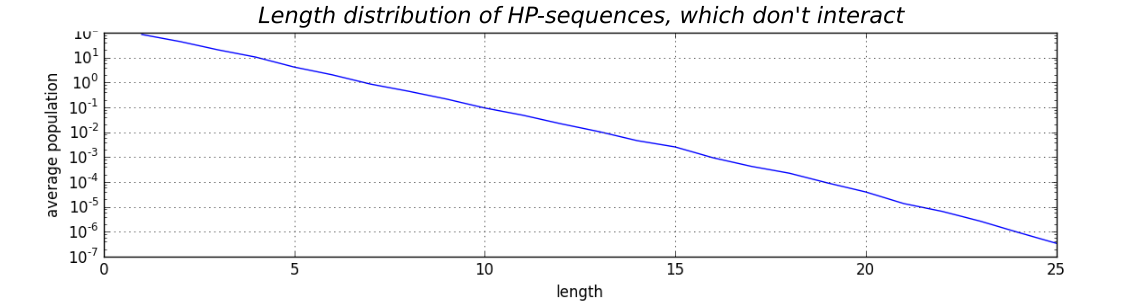
\includegraphics[width=0.95\textwidth]{pictures/flory.png} 
  \caption{We are dealing with an exponential length distribution. 
    Model described in \ref{sec:flory-derivation}}
  \label{fig:flory}
\end{figure}
\red{add another line with lower degradation constants}
Let us consider set up, which gives figure \ref{fig:flory}. 
This particular system is a throughput system. We have import of monomers and a sink. Polymers 
polymerize by monomer addition from one side. All bonds of the polymers are subject to random 
hydrolysis.

This model gives the following 
polymer abundance for the blue line:
\begin{equation}
  \frac{\pq{10mers}}{\pq{1mers}}\propto10^{-3},\qquad\frac{\pq{20mers}}{\pq{1mers}}\propto10^{-7}
\end{equation} 
For such a system, if we start with nano-molar concentrations of monomers, 40-mers will have 
concentrations $\propto 10^{-23} $ mol/L, which is just a few molecules per liter. 

We worked through several models of spontaneous polymerization, and all of they yield exponential 
or near-exponential length distribution.

\section{We use hydrophobic effect to solve Flory problem}

Hydrophobic effect is an effect which lays in the core of protein folding. It is mostly an 
entropic effect originating from the disruption of hydrogen bonds between water 
molecules by the nonpolar solute. \cite{Silverstein1998}. When hydrophobic molecules are placed in 
the water, water molecules form cage-like structures around them (see fig. \ref{fig:hydro-effect}). 
When hydrophobes come into contact, water molecules get released; this increases entropy and 
therefore decreases free energy. This decreases in free energy allows proteins keep a tight 
hydrophobic core.
\begin{figure}[h!]
  \centering
  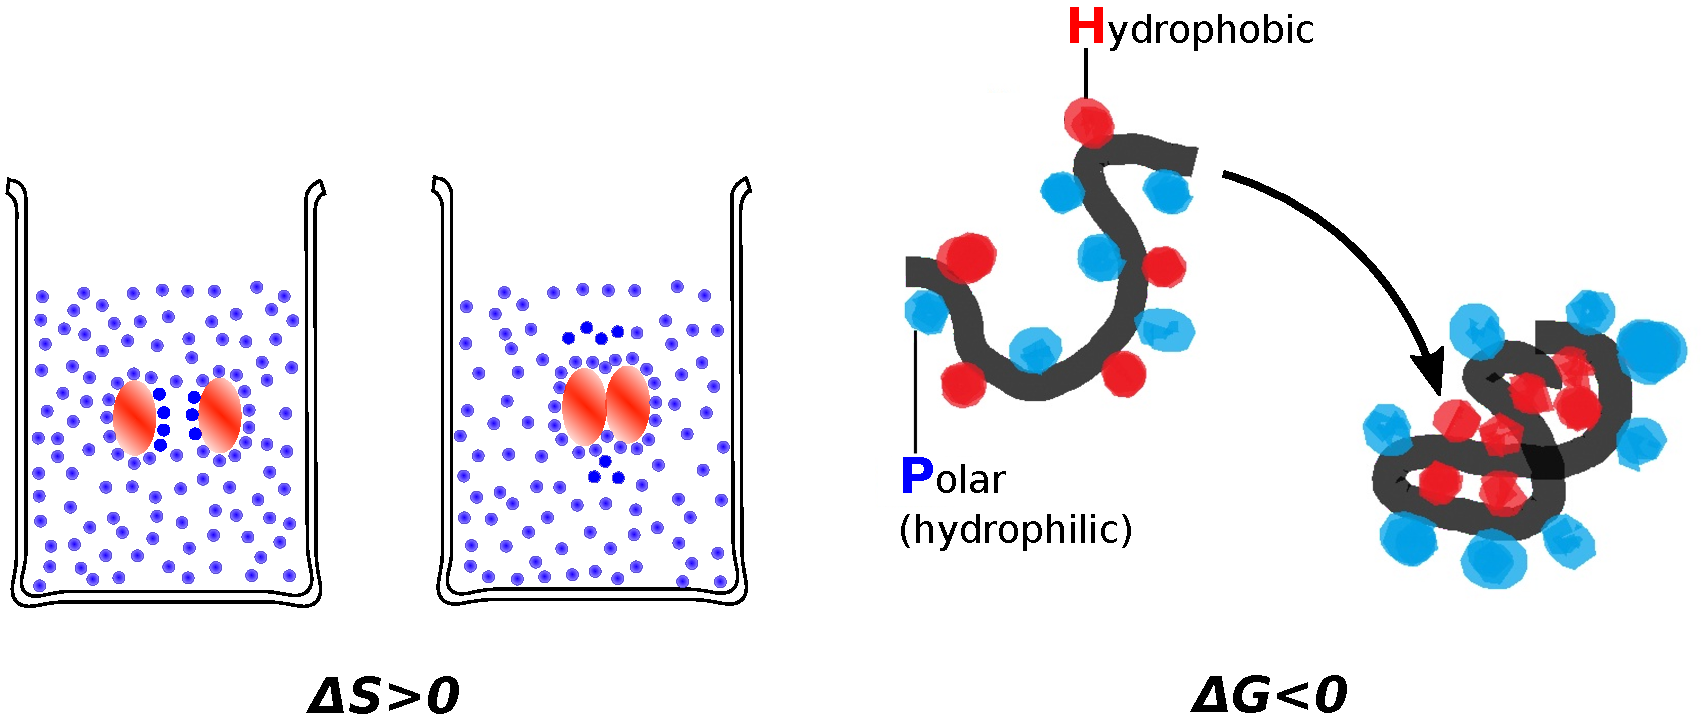
\includegraphics[width=0.7\textwidth]{pictures/hydrophobic-effect.pdf} 
  \caption{Hydrophobic effect is an entropic effect originating from the disruption of 
hydrogen bonds between water molecules by the non-polar solute.
When hydrophobic molecules are placed in the water, water molecules form cage-like 
structures around them. When hydrophobes come into contact, water 
molecules get released; this increases entropy and therefore decreases free energy. }
  \label{fig:hydro-effect}
\end{figure}

\subsection{We use HP model to represent prebiotic polymerization}
To describe effect of hydrophobic interaction on prebiotic polymerization, we adopt the HP model 
-- one of the simplest models of proteins; it's well studied and sequence space is well 
understood\cite{lau1989lattice,Chan1991,Miller1995,Yue1995,agarwala1997local}. While initially HP 
model was introduced as a model for proteins, we are indifferent to exact chemical nature of the 
prebiotic polymers and consider only principles of spontaneous polymerization.
\paragraph{HP model features:} 
\begin{itemize}
 \item It is a two dimensional square lattice model of protein folding
 \item It has 2 types of monomers: hydrophobic (H) and polar (P). 
 \item HP model has a folding code: presence of hydrophobic interaction makes some conformations 
of the same chain more energetically favorable than others. Moreover certain chains will have a 
unique conformation, which delivers free energy minimum. This conformations are called native 
states, and sequences, which have native state, are considered being capable of folding (see fig. 
\ref{fig:hp-model} ).
\end{itemize}

\begin{figure}[h!]
  \centering
  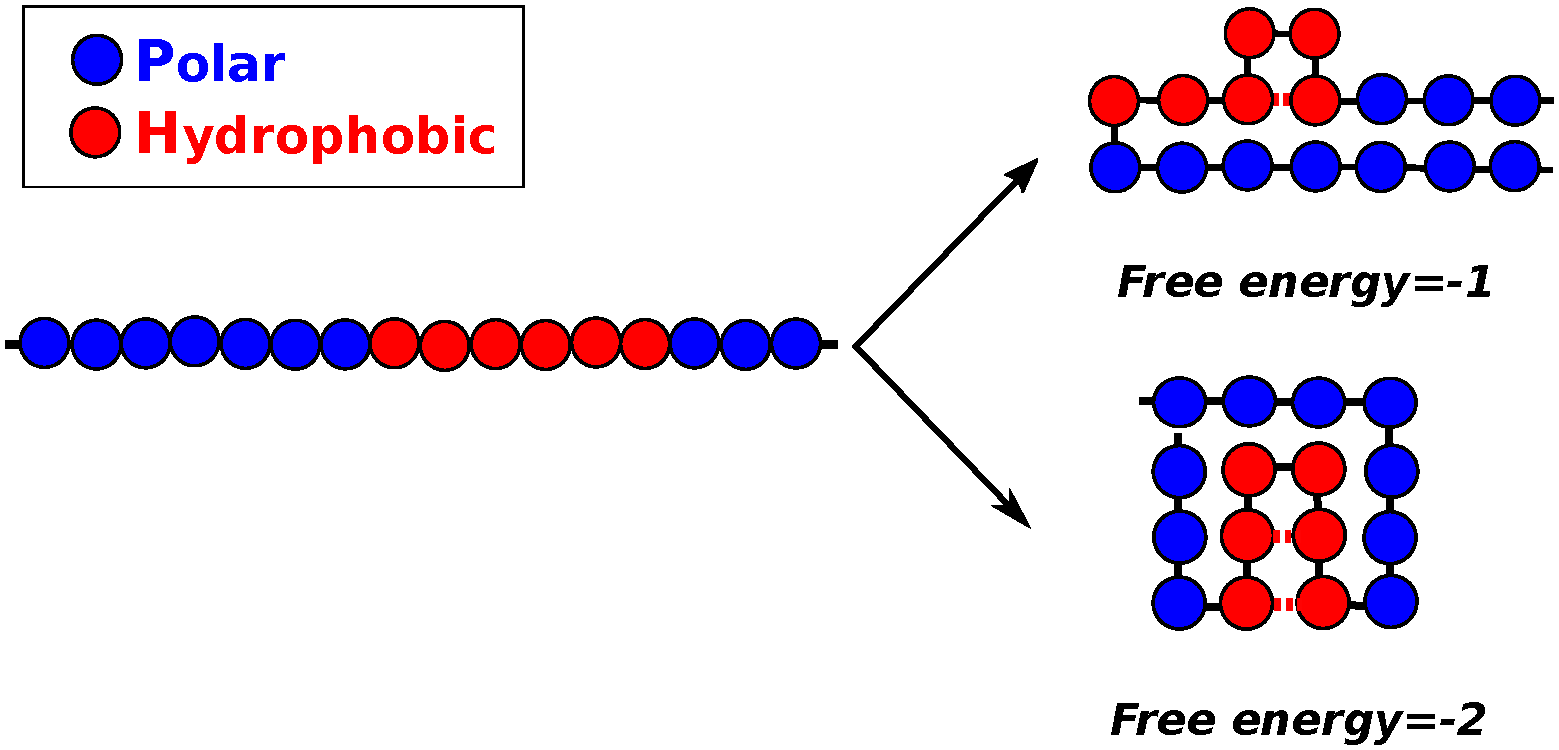
\includegraphics[width=0.6\textwidth]{pictures/hp-model.pdf} 
  \caption{}
  \label{fig:hp-model}
\end{figure}
Because of the ability to form hydrophobic contacts in water, even hetero-polymers that 
are as simple as HP-polymers will often fold up, even as short chains. 
While short HP chains will not necessarily have great stability qualities (they will often be 
fairly amorphous ``oil-drop''-like balls that are ensembles of conformations), some HP 
sequences will fold more uniquely than others. Latter will spend most of the time in the native 
state. And, what is important, it has been shown that a 
relatively large fraction of sequence space will fold to compact structures or compact ensemble 
structures\cite{lau1989lattice}.

\subsection{HP-foldamers can work as prebiotic catalysts}
Our central premise is that the same promiscuous hydrophobic interactions that can cause random 
HP heteropolymers to collapse into compact, folded, structures. However hydrophobic 
interaction will also cause polymer-polymer attraction and binding between molecules.  In some 
cases, a folded HP-polymers can provide a hydrophobic ``landing site'' for another HP polymer 
and/or another H monomer (see fig. \ref{fig:hp-catalysis}).  


When a folded chain has exposed hydrophobic monomers on its surface it can attract another chain 
with hydrophobes as well as activated hydrophobic monomer. Interaction between 3 of them localizes 
growing chain and next monomer (fig.\ref{fig:hp-catalysis}(a)). In addition to that, hydrophobic 
interaction also lowers activation barrier of the polymerization reaction, accelerating reaction 
this way.

One hydrophobic interaction is about $1-2kT$. Given that rate of catalysis is proportional to an 
exponent of the activation barrier, 3-4 hydrophobic interactions are enough to increase 
polymerization rate $\approx 100$ times (fig.\ref{fig:hp-catalysis}(b)). 
Of course, this is not a good rate compared to modern biochemical rates. However the very 
first catalysts don't have to be very efficient: their purpose is to create a driving force of 
evolution.

HP-catalysis drives addition of hydrophobes to hydrophobes. A seemingly logical conclusion would 
be that one will end up with purely hydrophobic polymers. However this is not true. Sequences 
capable of catalysis must have a relatively stable structure. Purely hydrophobic sequences don't 
have this property: they have very many conformational states with the same low free energy. 
Therefore they will spend a lot of time jumping between those states and their bonds will be 
affected by hydrolysis. They also will not be able serve as catalysts. Sequences with $50-80\%$ 
of hydrophobes, on the other hand, will have the most stable structures; they will 
be protected from hydrolysis and will be able to localize growing chain with the next added 
monomer.
\begin{figure}[h!]
  \centering
  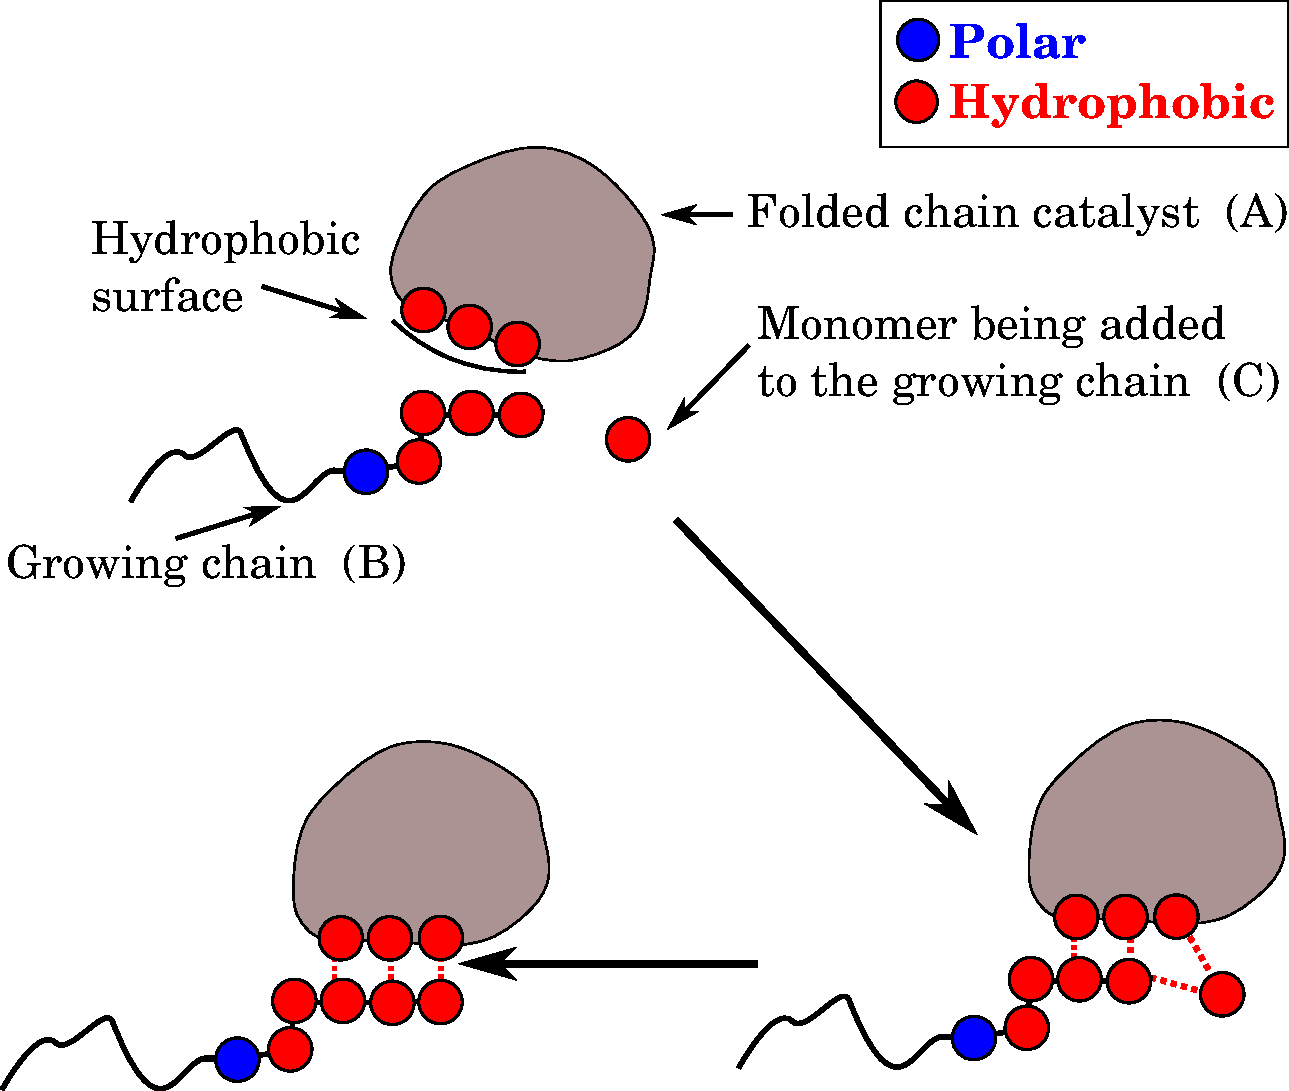
\includegraphics[width=0.85\textwidth]{pictures/hp-catalysis.pdf} 
  \caption{Catalyst catalyzes a growing of an unfolded hp-polymer. 
           Having just 3-4 hydrophobic contacts is enough to lower an 
           activation barrier for $\propto 100$ times at room 
           temperature.}
  \label{fig:hp-catalysis}
\end{figure}


\section{Materials and methods}\label{sec:mat}
\subsection{Simulations}\label{sec:mat-sim}
To test our hypothesis we performed direct stochastic simulations on several. We used 
\blue{PDMmod} method \cite{Bernatskiy}\footnote{C++ library and description can be found 
here: https://github.com/abernatskiy/pdmmod}. Stochastic simulations keep track of each 
molecular specie in the system. However simulations are limited due to computational reasons. First 
of all we have to explore conformational space of every polymer. This task is NP-hard (we use 
HPSandbox algorithm\cite{lau1989lattice,Dill2008} \footnote{Python implementation and description 
can be found here: http://hp-lattice.readthedocs.org/en/latest/}), so we had to limit 
maximum chain lengths to 25. We also try to keep total number of species in the low thousands, to 
avoid computational costs. We do it by introducing dilution parameter $d$: molecules are being 
removed from the system with probabilities $\propto d$. This mimics a protocell splitting and 
loose of materials due to it. Total number of molecules varies from simulation to simulation, 
however it mostly holds in the region \red{insert}.

We start our simulations with a small pool of monomers, usually below 100 molecules. 
\begin{itemize}
 \item We assume 
that there are enough of activated monomers in the system, so that their concentrations are 
constant. This way we don't have to track them in the simulations.
\item Polymers can therefore 
spontaneously grow with the rate $\ga$, which we put equal 1 for simplicity; all other rates are 
relative to the growth rate.
\item Activated monomers decay into regular ones with the rate $a\gg1$. This 
imitates input of food into the system. 
\item Dilution parameter $d$ varies from $\propto 0.01$ to 
$\propto 1$.
\item Hydrolysis has constant rate $d_h$ per bond; it varies from $\propto 0.01$ to $\propto 1$.
\item Folding and unfolding reactions happen very quickly with the rates $k_{unf}\gg1$ and 
$k_{unf}\cdot\exp(E_{native}/kT)$ correspondingly.
\item Catalysis rate is proportional to the exponent of hydrophobic energy $E_h$ and number of 
contacting hydrophobes $n_c$: $\ga\cdot\exp(E_{h}\cdot n_{c}/kT)$
\item Some experiments also include aggregation reactions for the long hydrophobic chains.
\end{itemize}
We looked at the lengths distribution in steady state. In order to account for stochastic effects 
we took average over several realizations. We also looked at the time evolutions of specific 
chains to investigate correlations between sequences and internal dynamics. The simulations were 
performed on Computing Cluster of Laufer Center. See \blue{appendix} for simulation details.

\paragraph{Experiment 1. Reproduction of Flory distribution.}
We started simulations with small pool of monomers (20 H and 20 P). We ran 30 identical  
simulations for 200 s each, with measurements taken every 0.1s. Steady state is being achieved 
around 30-50s. To calculate length distribution, we took one trajectory and calculated average 
over time over all time points after 100s; so we got 1000 time points for every chain length, over 
which we averaged. The rate of conversion of activated monomers into regular ones is $a=100$. We 
took dilution rate of $d=0.5$. We ran experiments for 2 hydrolysis rates: $d_h=0.3$ and $d_h=0.03$.
We varied hydrolysis and dilution rates. Experiments with $d_h=0$ reproduce accurate exponential 
curves; adding hydrolysis, however, slows down distribution around short lengths. This effect is 
due to constant concentration of activated monomers: there's no competition for ``food''. This 
enriches population of short chains, however doesn't affect longer chains significantly, leaving 
their distribution nearly exponential.

\paragraph{Experiment 2. Study how folding affects length distributions.}
In addition to the parameters of the  experiment 1 we also added non-zero hydrophobic energy and 
introduced folding and unfolding reactions.
 Hydrophobic energy is taken $E_h=2kT$ and rate of unfolding is $k_{unf}=100$. We varied parameters 
around given values and didn't notice qualitative changes of the system's behavior.
From the figure \ref{fig:sim.flory-fold} in section \ref{sec:res} we can see 
that presence of folding doesn't affect length distribution significantly.

\paragraph{Experiment 3. Introduction of HP-catalysis.}
In addition to folding in this \textit{in-silico} experiment we introduced interaction between 
proteins. All parameters are as above. We varied parameters of the simulations, and noticed 
significant stability of the length distribution towards change of $d_h$ and $d$. distribution is 
sensitive towards hydrophobic energy, as expected. Chain length distribution has a noticeably 
non-exponential behavior in the region when $E_h= 1-3 kT$

\paragraph{Experiment 4. HP-catalysis and aggregation.}
Short description


\paragraph{Experiment 5. Study of internal dynamics.}
Short description




\section{Results and discussion}\label{sec:res}
\paragraph{Simulation: folding.} Presence of folding reactions and absence of catalysis ones 
relationship between abundance and length at steady state follows exponential distribution for 
longer chains and is slower than exponential for short chains. While presence of folding makes 
some of the folded sequences get higher than average for their length populations, these 
populations are never more than few-fold of average population of regular sequences and don't 
change nature of the distribution.
\begin{figure}[h!]
  \centering
  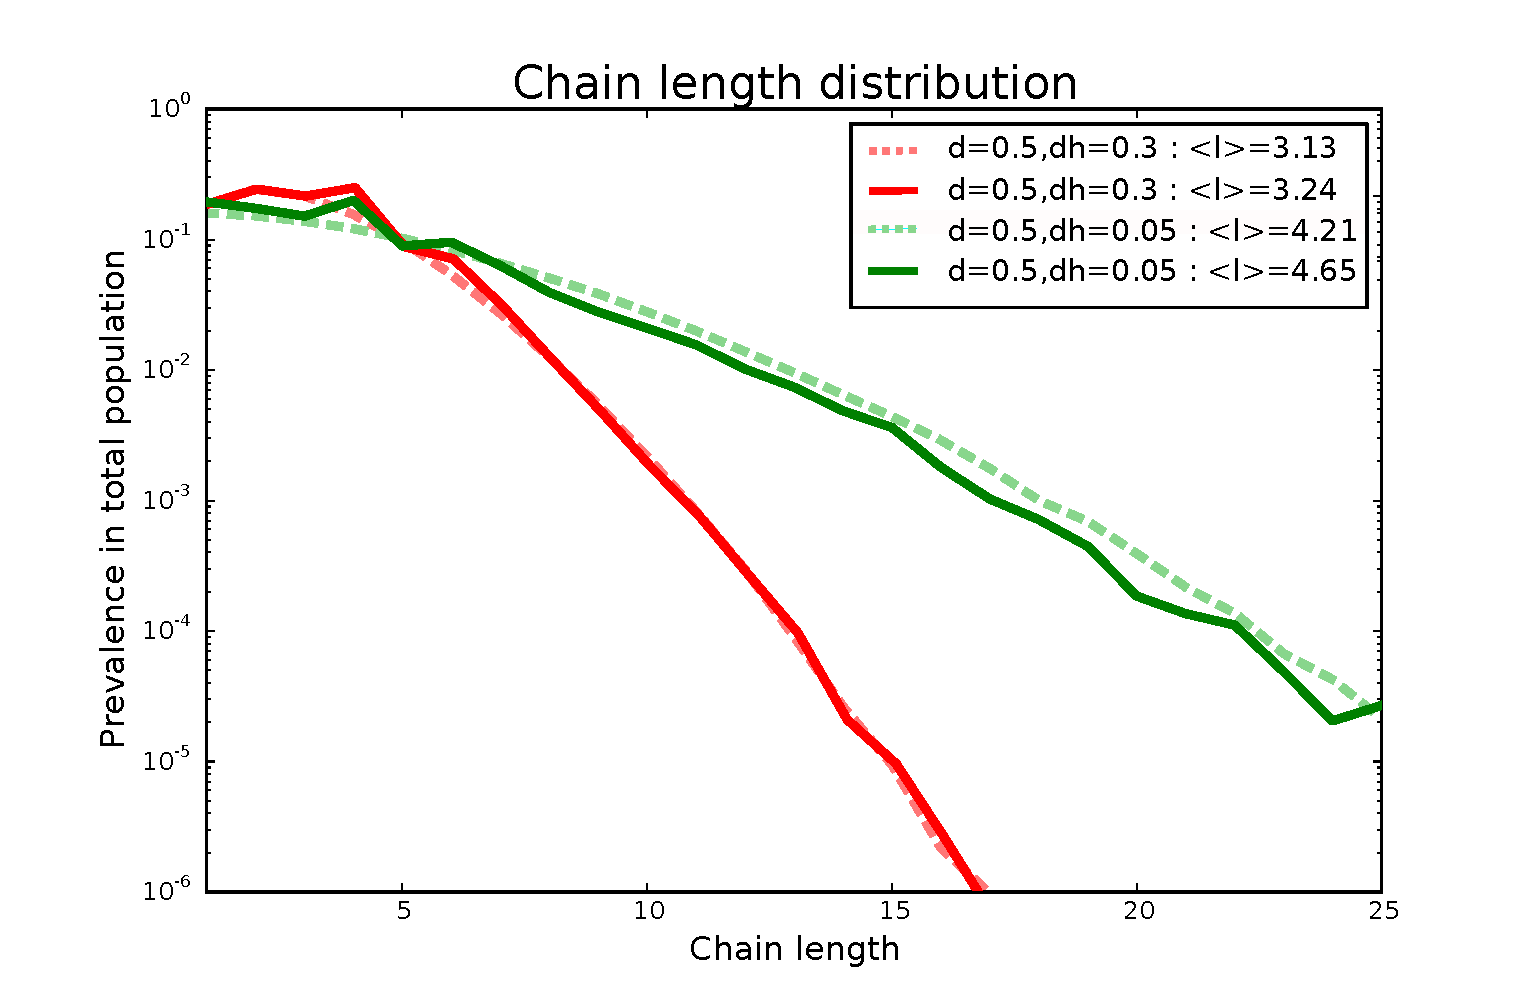
\includegraphics[width=0.85\textwidth]{pictures/flory-and-fold.pdf} 
  \caption{Dashed lines represent polymerization without folding or catalysis. Solid lines 
correspond to simulations run with folding but without catalysis. For details of simulations see 
section \ref{sec:mat-sim}, Experiment 2. }
  \label{fig:sim.flory-fold}
\end{figure}

\paragraph{Simulation: folding and HP-catalysis.} Presence of catalysis in the system skews the 
distribution significantly, and while it leaves average chain length about the same it brings 
substantial excess of long sequence compared to the cases without catalysis\ref{fig:sim.flory-hp}. 
The system is fairly stable towards hydrolysis and dilution parameters. It allows for 1 order of 
magnitude change in those parameters without significant change in the behavior of the system. 
Sequences responsible for the skew of the distribution are few in numbers they all are catalysts 
and have long stretches of hydrophobs, which also means that they are products of catalysis. In 
the figure \ref{fig:example1} there examples of several sequences. The lines represent average 
over 30 time evolutions. For this particular experiment, concentration of monomers at steady 
state is $\propto 100$. Most of the longer sequences have average populations $\ll 1$. However for 
the most of the chain lengths there are few sequences, which dominate populations significantly.
\begin{figure}[h!]
  \centering
  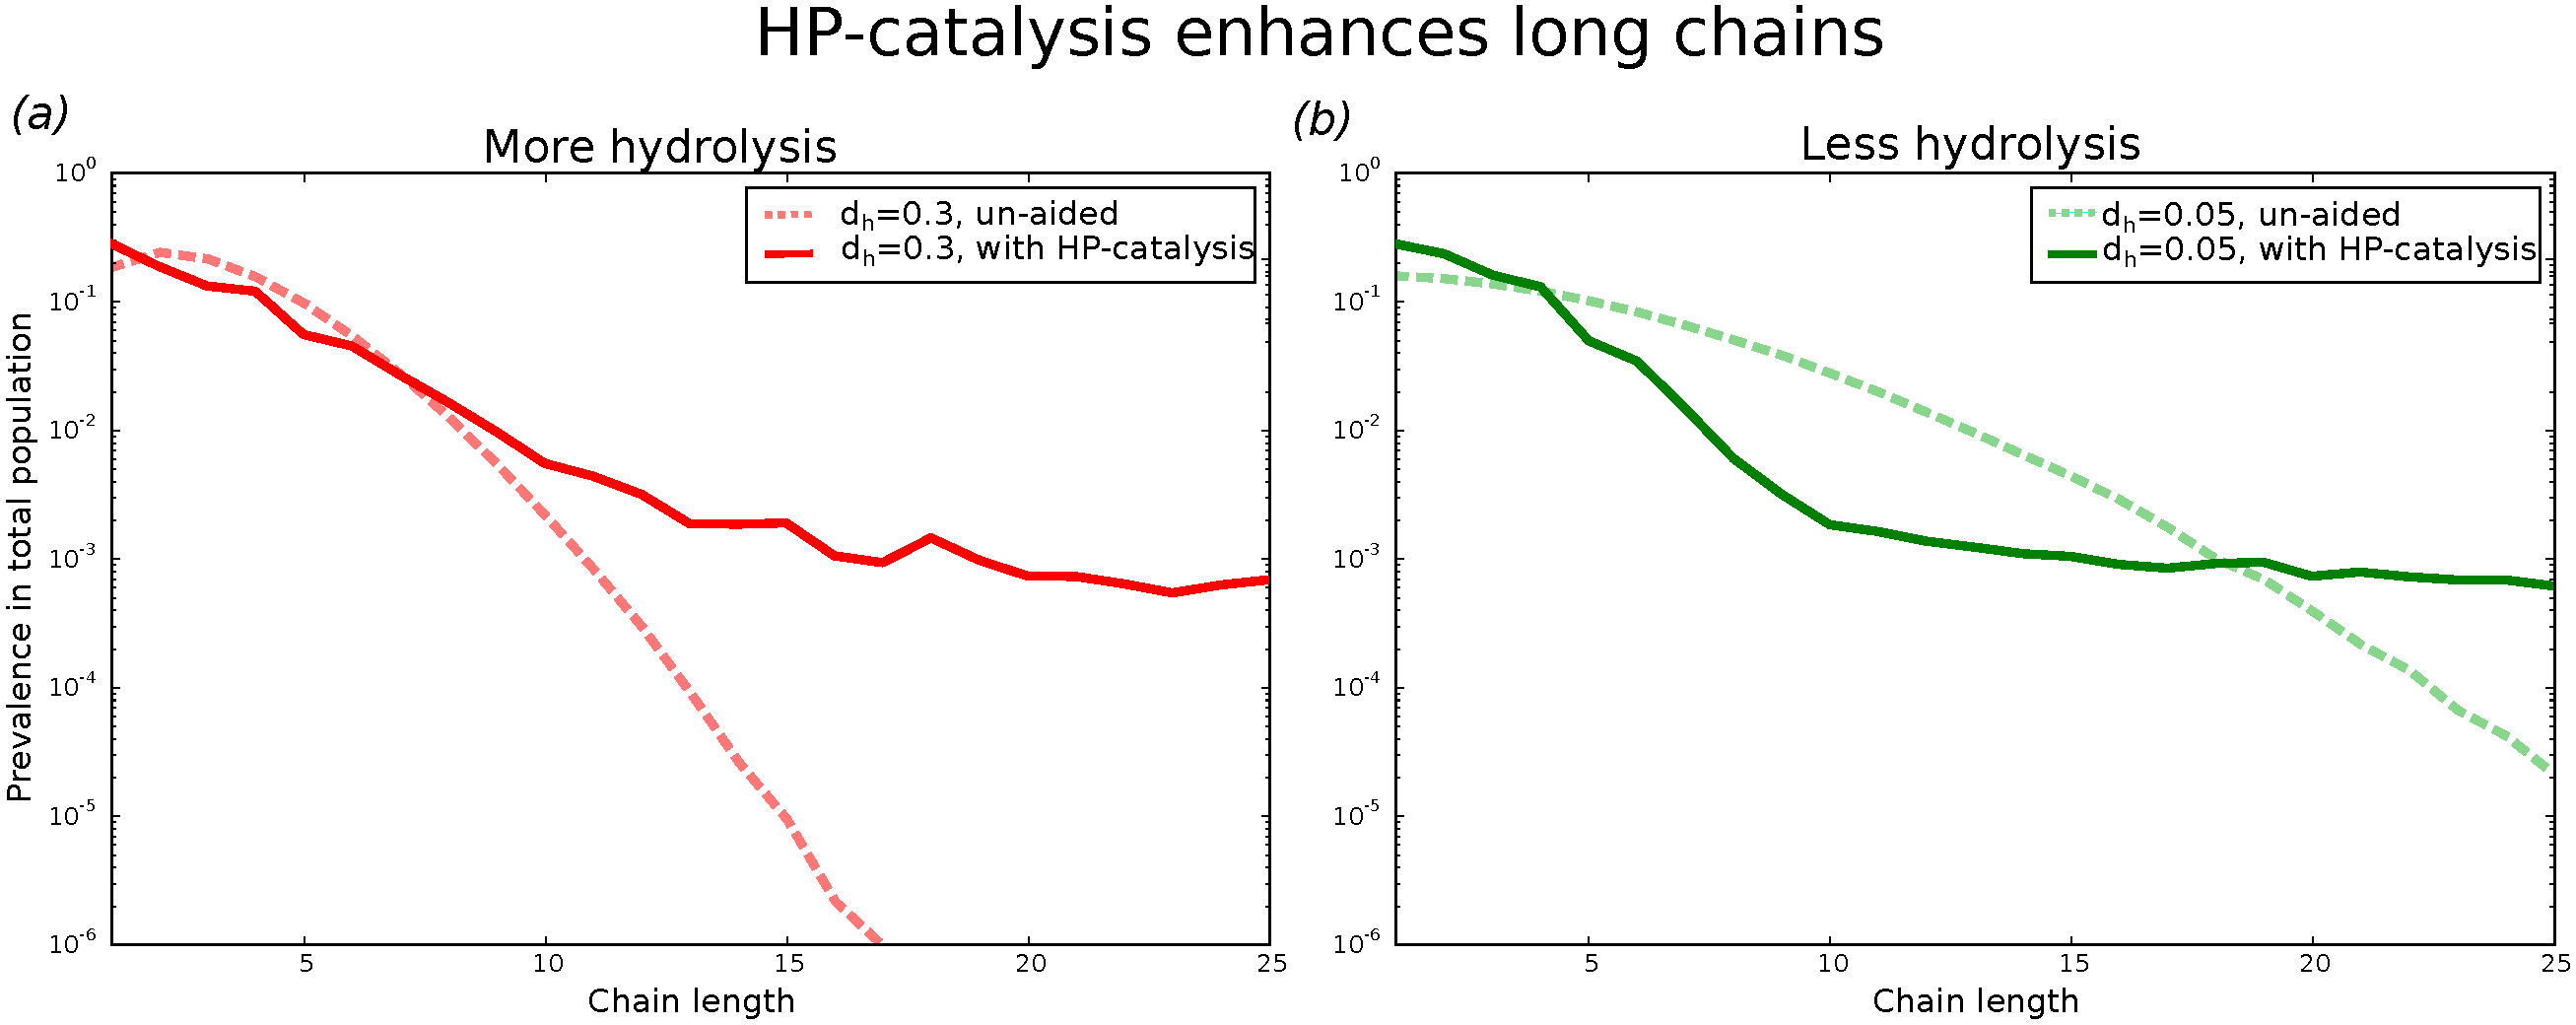
\includegraphics[width=0.85\textwidth]{pictures/flory-and-hp.pdf} 
  \caption{Dashed lines represent polymerization without folding or catalysis. Solid lines 
correspond to simulations run with folding and catalysis reactions on. For details of simulations 
see \ref{sec:mat-sim}, Experiment 3. }
  \label{fig:sim.flory-hp}
\end{figure}

\begin{figure}[h!]
  \centering
  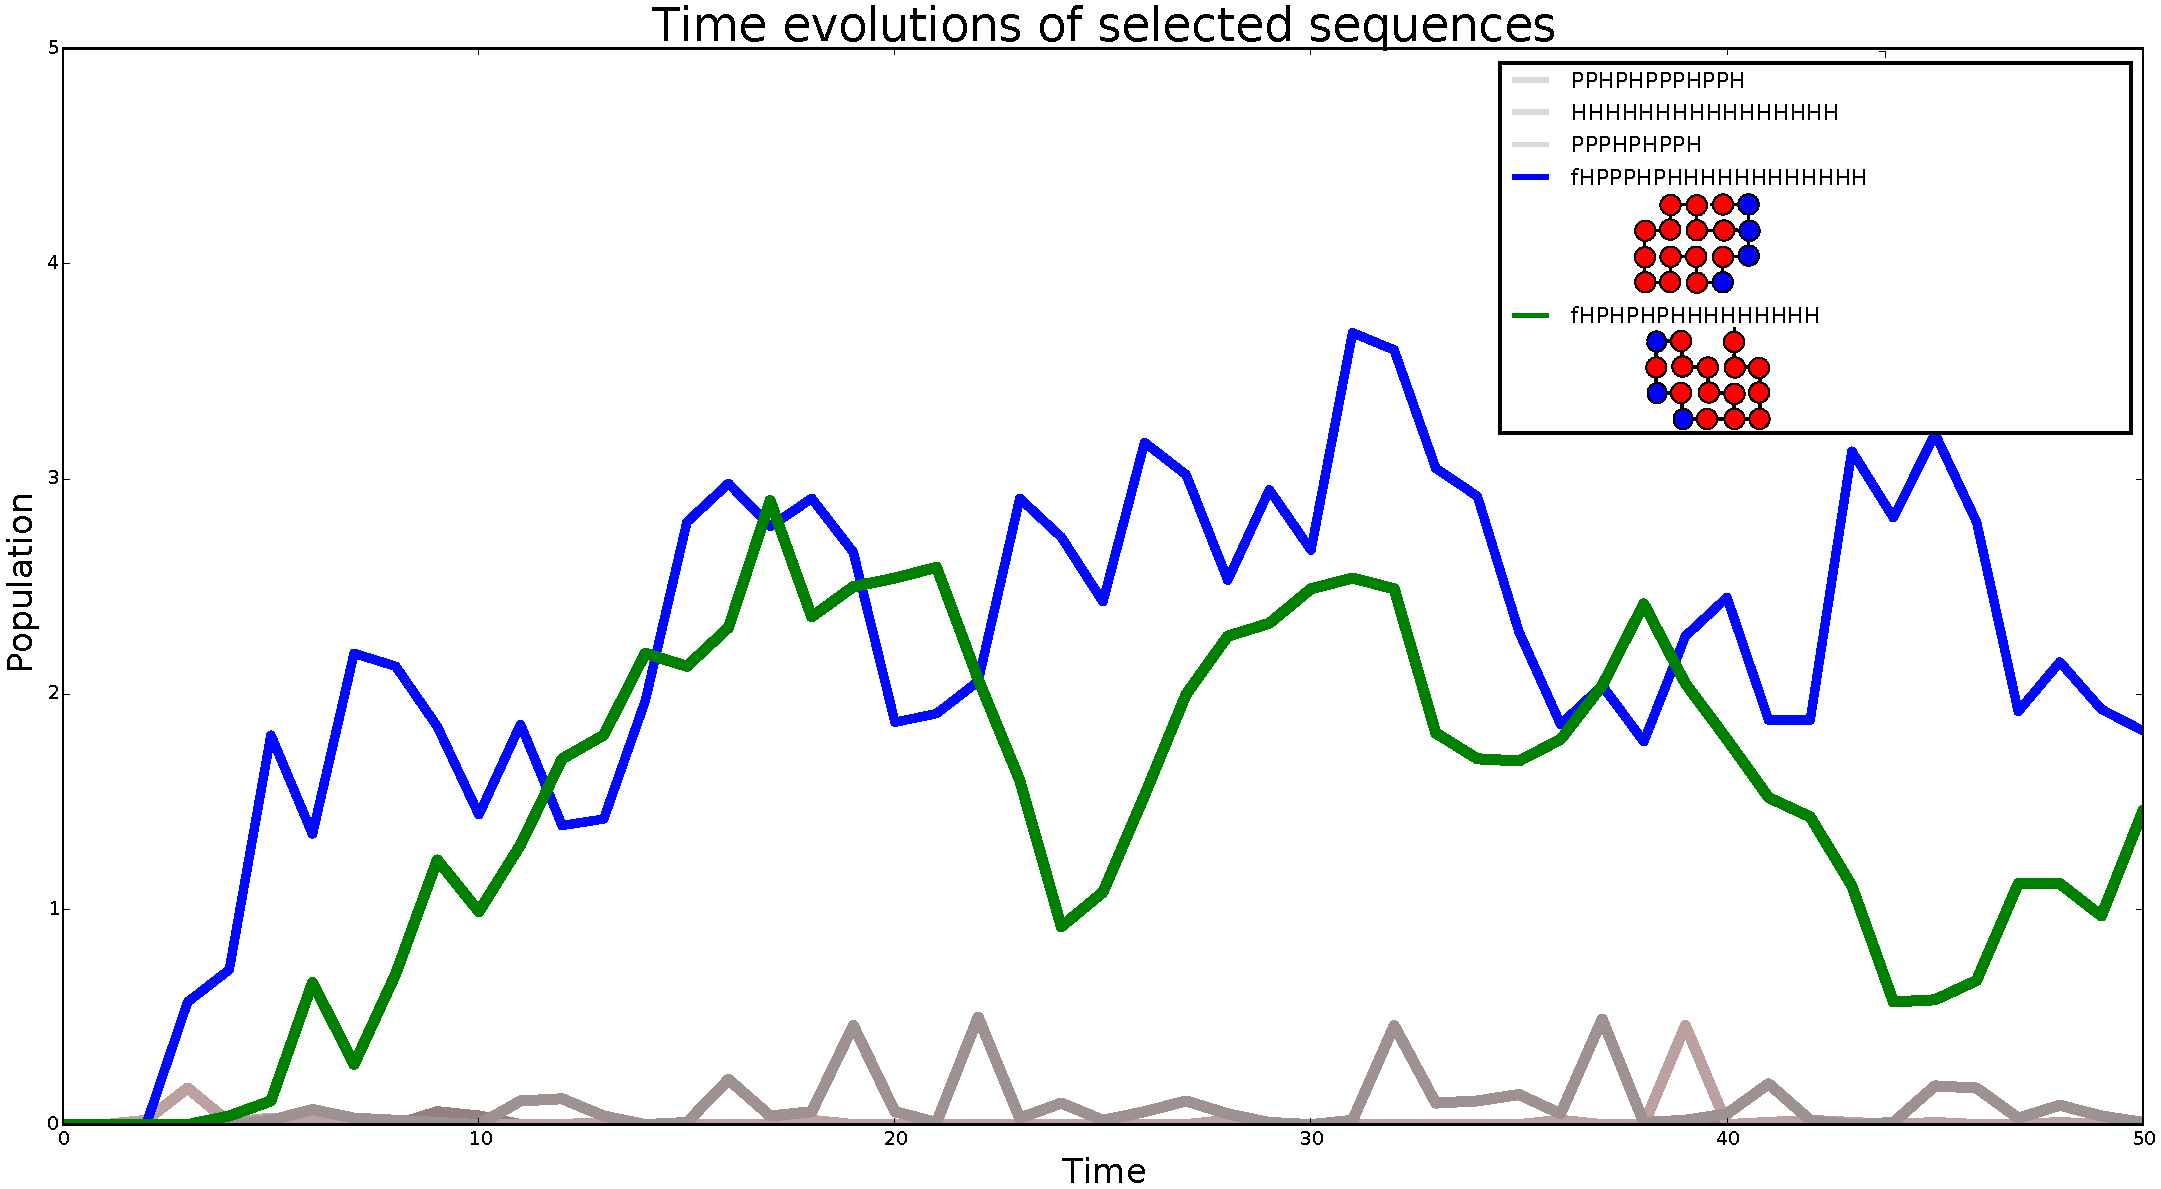
\includegraphics[width=0.85\textwidth]{pictures/example1.pdf} 
  \caption{Some examples of dominating autocatalytic sequences. Gray lines represent regular 
non-catalytic sequence. structures on the right are native structures of autocatalytic sequences. }
  \label{fig:example1}
\end{figure}

\red{Some discussion on what it means and that it is still not enough for a proper inheritance and 
evolution, however it allows us to get to longer sequences, some of which can be ``magical''.}



 \newpage
\appendix
\section{Flory problem derivation}\label{sec:flory-derivation}
% Suppose one has a plenty of monomers either in closed reservoir or in the system that allows 
% import of monomers and waste output. Suppose there are also two competing mechanism acting upon 
% the system: 
% \par (a) Growth: reactions like
% \begin{itemize}
%   \item (Activated) monomer addition
%   \item Ligation of two oligomers
% \end{itemize}
% \par (b) Degradation: reactions like
% \begin{itemize}
%   \item Full degradation/leaving a vesicle/dilution
%   \item Hydrolysis of bonds of polymers.
% \end{itemize}
% In systems like these the steady state distribution of length will be exponential
% Rate constants: growth=1, import=100, degradation=0.1

\section{Simulation details}



 \bibliography{/data/research/31.mendeleyBibtex/Origins}
  \bibliographystyle{unsrt}


\end{document}
